\documentclass[12pt]{article}

\usepackage[margin=1.25in]{geometry}
\usepackage{amsmath,amssymb}
\usepackage{booktabs}
\usepackage{graphicx}
\usepackage[hidelinks]{hyperref}
\usepackage[round]{natbib}
\usepackage{setspace}

\doublespacing
\emergencystretch=3em
\renewcommand{\ttdefault}{cmtt}

\title{Spherical Splits for Decision Trees and Random Forests: A Short Note}
\author{}
\date{}

\begin{document}
\maketitle

\begin{abstract}
Classical decision trees split covariate space with coordinate thresholds,
which creates rectangular recursive partitions. This note studies a simple
alternative in which a node sends observations left or right according to
whether they lie inside a learned hypersphere. The construction preserves the
usual impurity-based tree architecture while replacing some threshold questions
by distance-to-center questions. We describe the split rule for a data matrix
and response vector, show that distant sphere centers recover linear frontiers
locally, and note that CART cost-complexity pruning applies without changing
the pruning criterion. Exploratory benchmarks on PMLB datasets suggest that
spherical random forests can improve mean classification performance, although
the current split search is slower and the same advantage is not observed for
regression or for single trees.
\end{abstract}

\noindent\textbf{Keywords:} decision trees; random forests; classification;
spherical splits; recursive partitioning.

\section{Introduction}

Let $\mathbf{X}\in\mathbb{R}^{n\times p}$ be a data matrix, with rows
$\mathbf{x}_i^\top$, and let $\mathbf{y}$ be a class label or response vector.
Decision trees remain useful for such tabular classification and regression
problems because they are nonparametric, interpretable, and easy to ensemble.
Their usual form, however, fixes a strong geometry. At each internal node,
CART-style trees, as introduced by Breiman, Friedman, Olshen, and Stone (1984),
select a feature index $j$ and a threshold $a$, then split observations
according to $x_{ij}\le a$ or $x_{ij}>a$. Recursively, this creates rectangular
cells.

Rectangular cells are natural when the signal is sparse and coordinate-aligned.
They are less economical when the target depends on membership in an area
around a center. In classification, a class may correspond to a compact region
or cluster; in regression, a response surface may change near a centroid or
prototype. An axis-aligned tree can approximate such a region, but it may need
many cuts. A spherical split can isolate the same type of region directly.

The resulting rule can also be easier to read than an oblique split in some
settings. An oblique rule asks whether a weighted linear combination of
covariates exceeds a threshold, as in the OC1 system of Murthy, Kasif, and
Salzberg (1994). A spherical rule asks whether an observation lies within
radius $r$ of a center $\mathbf{c}$. When
the active covariates define a meaningful metric space, this is a
local-neighborhood statement. For example, with projected latitude and
longitude, a split describes membership in a circular region around a
geographical point. This interpretation depends on scaling and on the metric,
but it can be more direct than an abstract linear score.

This short note makes three points. First, spherical splits define a simple
finite impurity search that can be inserted into ordinary tree induction.
Second, they interpolate geometrically between radial rules and linear
frontiers. Third, post-hoc CART pruning applies without changing the pruning
criterion. The empirical results are presented as exploratory evidence, not as
a dominance claim.

\section{Spherical split rule}

At a node, let $S\subseteq\{1,\ldots,p\}$ be the active feature set. A spherical
split is determined by a center $\mathbf{c}\in\mathbb{R}^{|S|}$ and a radius
$r\ge 0$:
\[
    \|\mathbf{x}_{iS}-\mathbf{c}\|_2^2 \le r^2.
\]
Observations satisfying the inequality are sent to one child and the remaining
observations to the other. The pair $(\mathbf{c},r)$ is chosen to maximize the
same impurity decrease used in ordinary tree induction, such as Gini decrease
for classification or variance reduction for regression.

The implementation studied here uses finite candidate sets. Candidate centers
are generated from global centers, target-conditional centers, observed points,
pairwise midpoints, local Gaussian perturbations, and farther radial
perturbations. For each candidate center, the candidate radii are the Euclidean
distances from the center to the node samples. Thus the geometry changes, but
the optimization remains a finite sequence of impurity comparisons.

Figure~\ref{fig:frontiers} compares axis-aligned, oblique, and spherical
partitions on two-dimensional examples. The spherical panels show internal
circles; terminal regions are intersections of recursive inside/outside
decisions.

\begin{figure}[t]
    \centering
    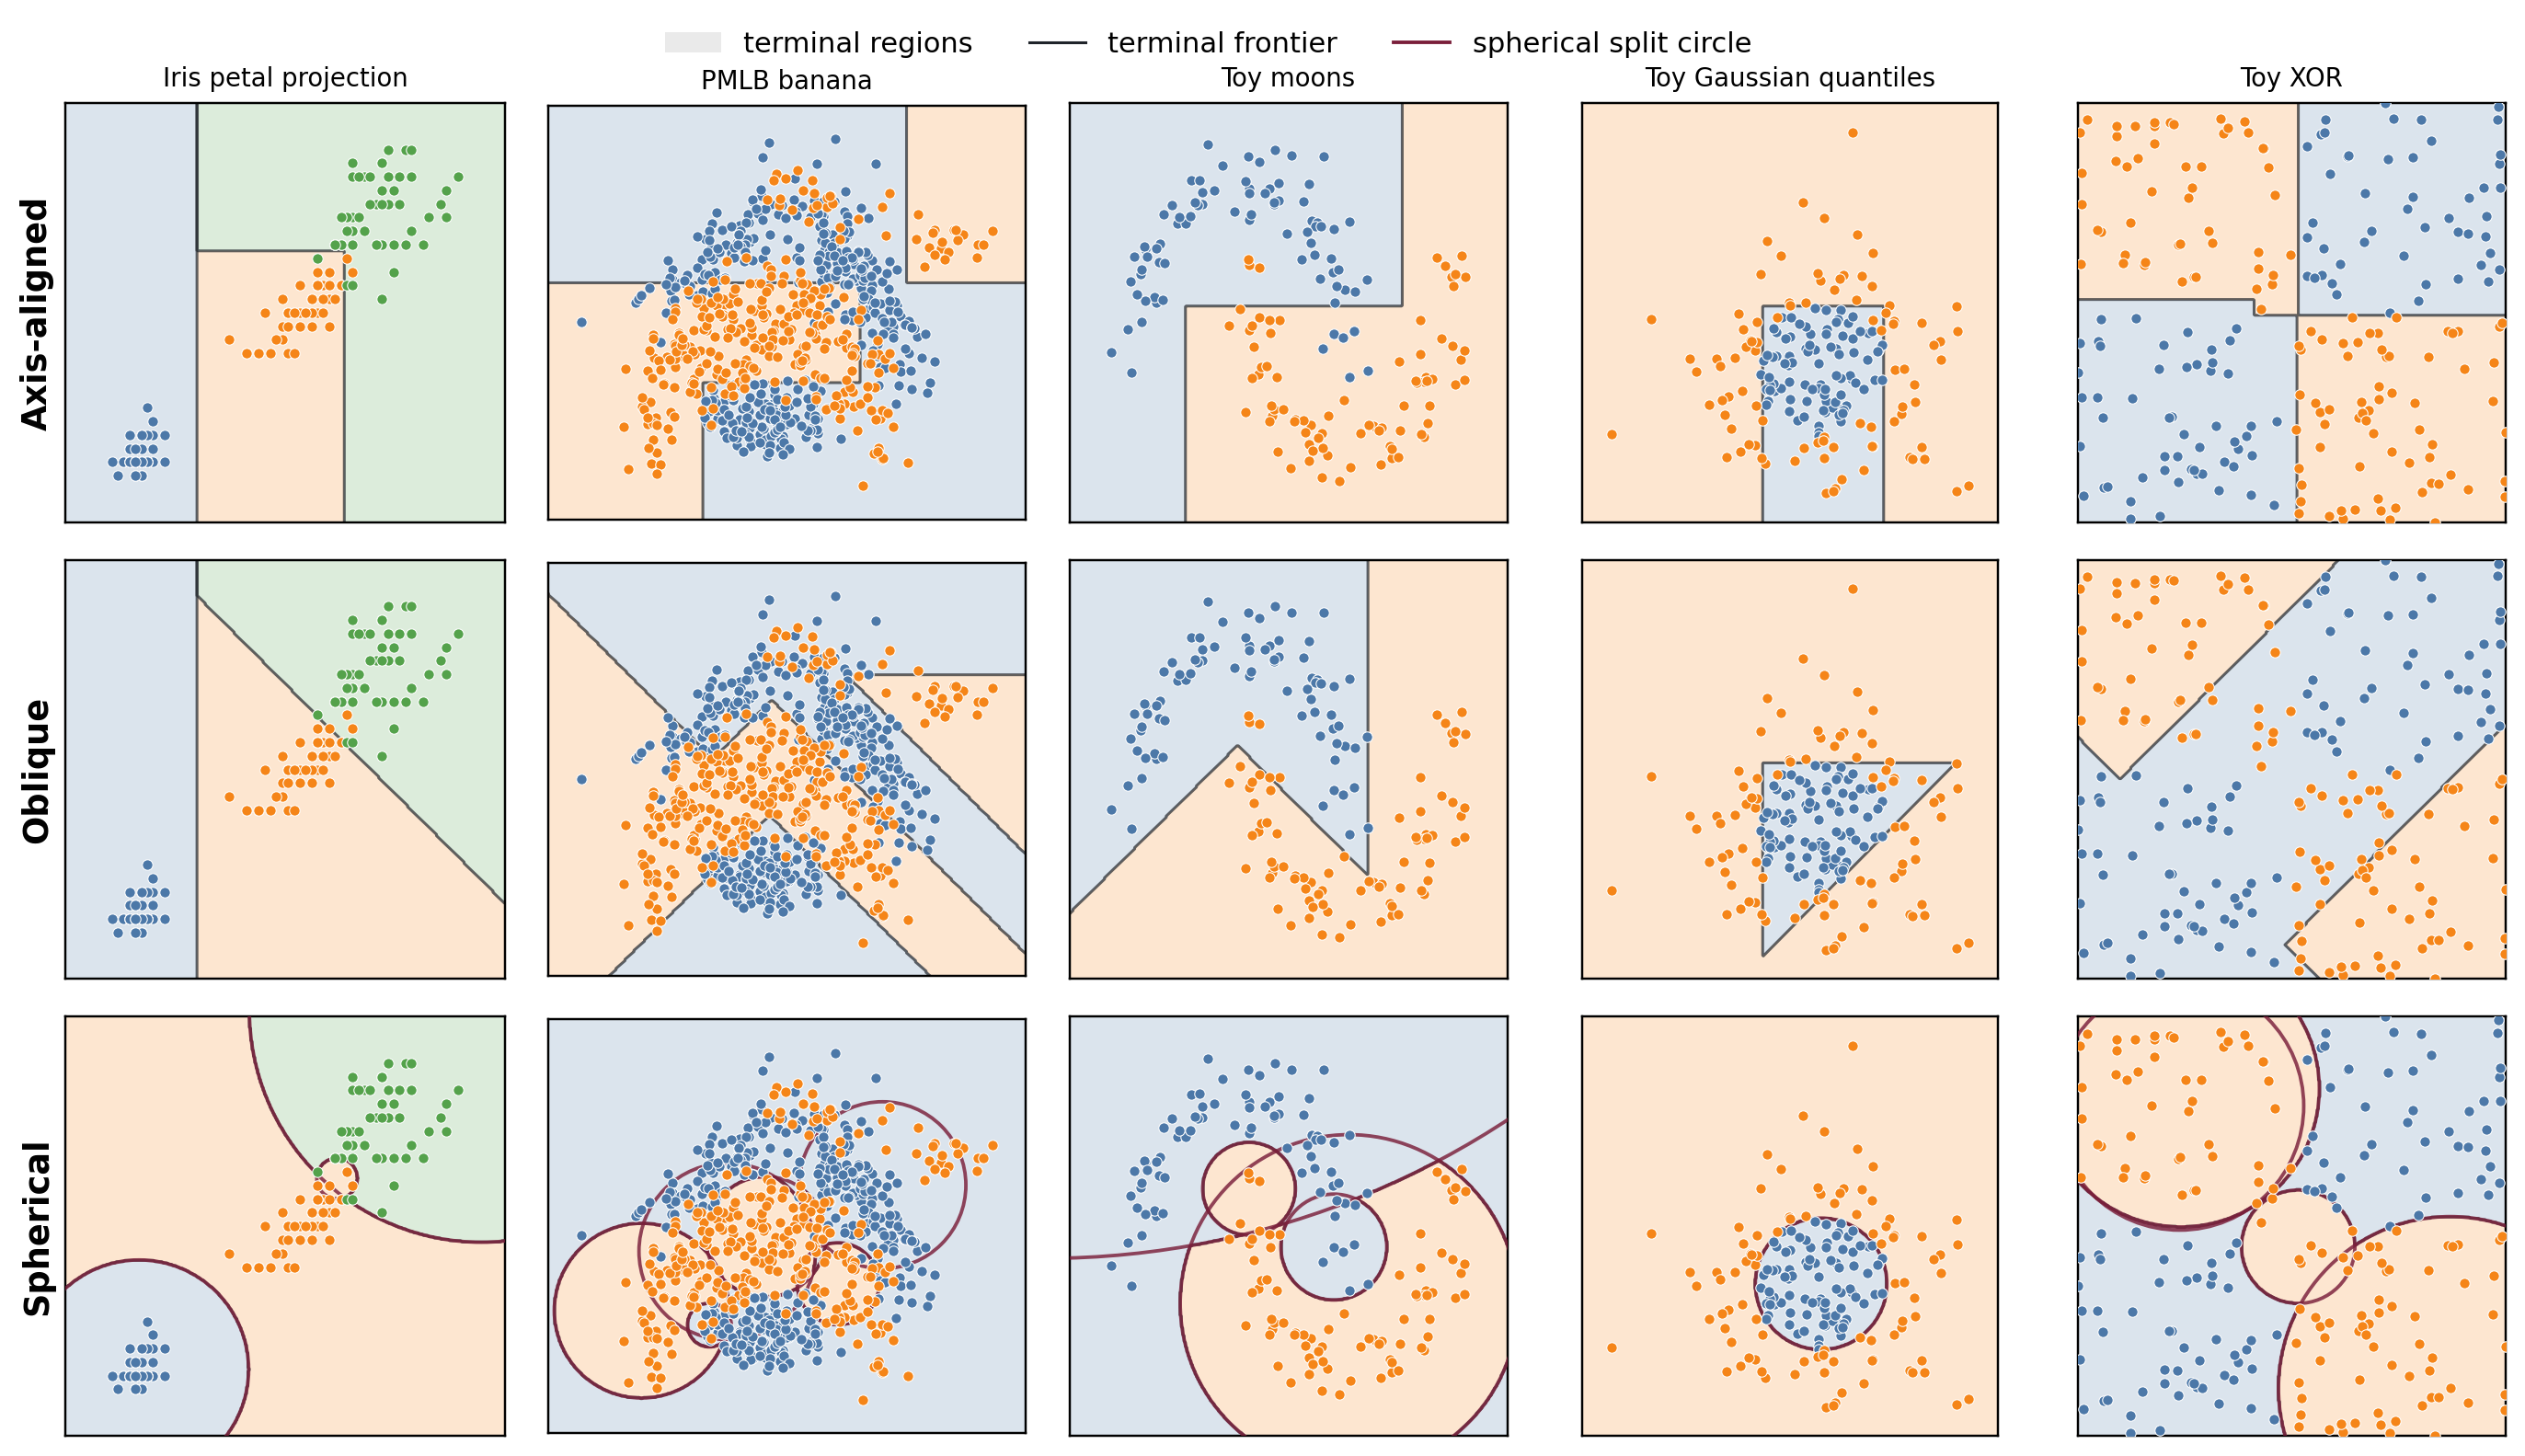
\includegraphics[
        width=4.8in,
        height=6.8in,
        keepaspectratio
    ]{Figure_1_axis_oblique_spherical.png}
    \caption{Two-dimensional decision regions learned by shallow
    axis-aligned, oblique, and spherical trees. Black curves are terminal
    decision frontiers; burgundy circles are internal spherical split
    boundaries.}
    \label{fig:frontiers}
\end{figure}

\section{Geometry and pruning}

The most direct case for spherical splits is radial or local structure. If the
target changes when $\mathbf{x}$ enters a ball around $\mathbf{c}$, then one
spherical split can represent that event. A rectangular tree must approximate
the same ball by coordinate cuts.

Spherical splits also recover linear frontiers as a local limit. Let
$\mathbf{u}\in\mathbb{R}^p$ satisfy $\|\mathbf{u}\|_2=1$, fix
$t\in\mathbb{R}$, let $R$ be large enough that $R^2-2Rt\ge0$, set
$\mathbf{c}=R\mathbf{u}$, and choose
\[
    r_R^2 = R^2 - 2Rt.
\]
Then
\[
\begin{aligned}
    \|\mathbf{x}-R\mathbf{u}\|_2^2 \le r_R^2
    &\Longleftrightarrow
    \|\mathbf{x}\|_2^2 - 2R \mathbf{u}^{\top}\mathbf{x} + R^2
    \le R^2 - 2Rt \\
    &\Longleftrightarrow
    \mathbf{u}^{\top}\mathbf{x}
    \ge t + \frac{\|\mathbf{x}\|_2^2}{2R}.
\end{aligned}
\]
On any bounded region $\|\mathbf{x}\|_2\le B$, the final term is at most
$B^2/(2R)$. Hence the spherical split converges locally to the halfspace
$\mathbf{u}^{\top}\mathbf{x}\ge t$ as the center is moved far away. Taking
$\mathbf{u}$ to be a coordinate vector recovers an axis-aligned split in the
same limiting sense.

A leaf at depth $d$ is an intersection of at most $d$ sets, each either a ball
or the complement of a ball. Spherical-tree leaves are therefore
semi-algebraic cells defined by quadratic inequalities. In two dimensions their
boundaries are circular arcs; in higher dimensions they are hyperspherical
patches. This differs from axis-aligned boxes and oblique polyhedra, and it can
represent annuli or shells compactly.

Cost-complexity pruning adapts directly. CART pruning selects subtrees by
minimizing
\[
    R_\alpha(T)=R(T)+\alpha|\widetilde{T}|,
\]
where $R(T)$ is the empirical leaf risk and $|\widetilde{T}|$ is the number of
terminal nodes \citep{breiman1984cart}. Once a spherical tree has been grown,
this criterion depends only on topology, leaf predictions, leaf risks, and leaf
count. It does not depend on the internal split geometry. The usual
weakest-link pruning sequence and validation choice of $\alpha$ can therefore
be used unchanged.

\section{Exploratory benchmark}

We implemented spherical trees and spherical random forests in a
\texttt{treeple}-based prototype. We compared them with axis-aligned CART and
random forests, as well as oblique trees and forests. The benchmark used
complete PMLB datasets of Olson, La Cava, Orzechowski, Urbanowicz, and Moore
(2017) that ran without errors. Features were imputed and standardized. The
comparison used three cross-validation folds, 50 trees for forests, 500
spherical center candidates per node, all data-induced radii for each candidate
center, validation-selected pruning for single trees, and unpruned forests.
Large datasets were capped at 1000 sampled observations. The final comparison
contained 249 complete datasets and 38 skipped datasets or fetch/model errors.

\begin{table}[t]
    \centering
    \caption{Mean performance and fit time over complete datasets. The primary
    score is balanced accuracy for classification and $R^2$ for regression.}
    \label{tab:benchmark}
    \begin{tabular}{llrr}
        \toprule
        Task & Model & Score & Fit time (s)\\
        \midrule
        Classification & Spherical random forest & 0.765 & 9.850\\
        Classification & Random forest & 0.738 & 0.137\\
        Classification & Oblique random forest & 0.737 & 0.154\\
        Classification & CART & 0.722 & 0.074\\
        Classification & Oblique tree & 0.706 & 0.136\\
        Classification & Spherical tree & 0.688 & 4.132\\
        \midrule
        Regression & Random forest & 0.717 & 0.384\\
        Regression & Oblique random forest & 0.700 & 0.434\\
        Regression & Spherical random forest & 0.665 & 20.533\\
        Regression & CART & 0.521 & 0.078\\
        Regression & Oblique tree & 0.391 & 0.093\\
        Regression & Spherical tree & 0.262 & 7.516\\
        \bottomrule
    \end{tabular}
\end{table}

The salient empirical pattern is the classification performance of spherical
forests. In this exploratory benchmark, spherical random forests obtained the
best mean classification score among the compared forest methods. The advantage
does not appear generally in regression, where ordinary and oblique forests
remain stronger. Nor does it appear on average for single trees. This suggests
a specific use case: high-variance spherical split candidates may be useful
when stabilized by ensembling, especially in classification problems with local
or cluster-like structure.

\begin{figure}[t]
    \centering
    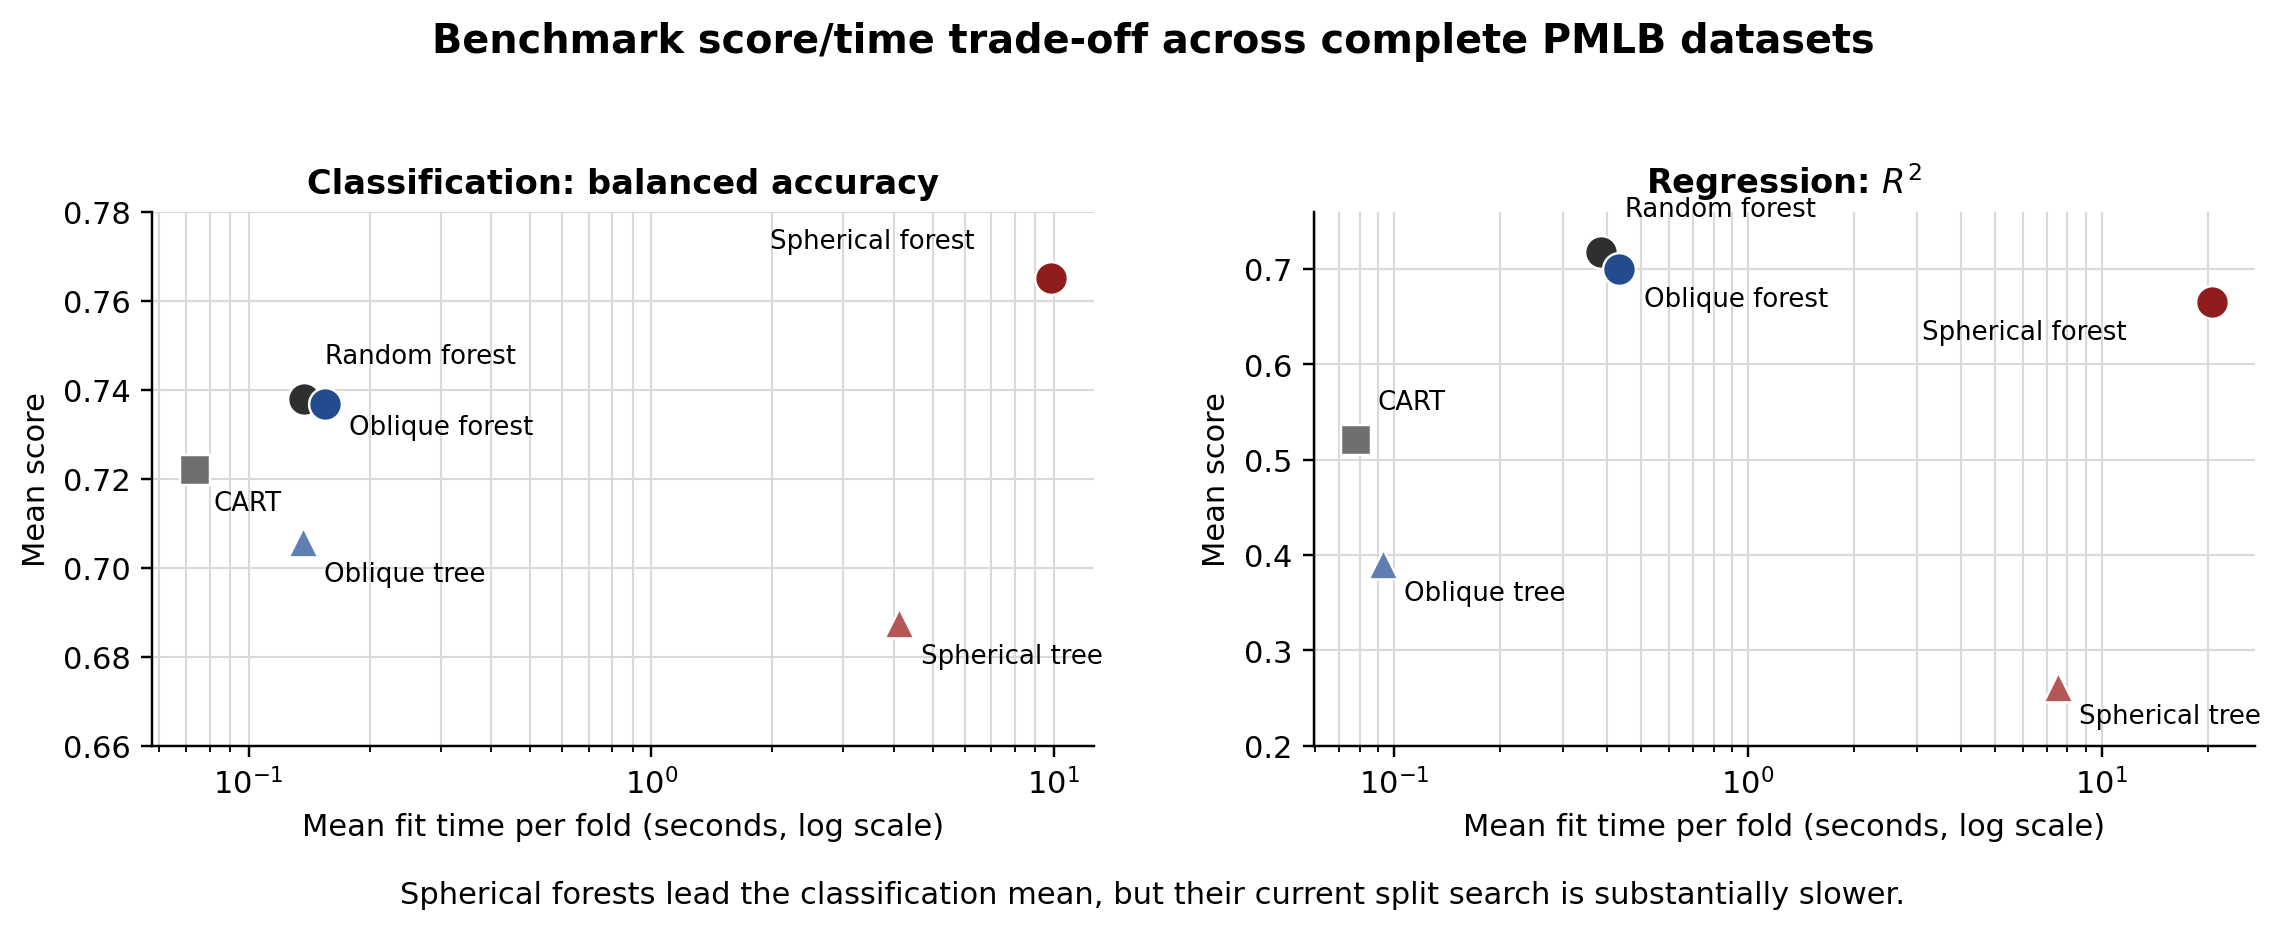
\includegraphics[
        width=4.8in,
        height=3.0in,
        keepaspectratio
    ]{Figure_2_score_time_tradeoff.png}
    \caption{Mean score and mean fit time over complete PMLB datasets. The
    current spherical split search improves the classification mean for forests
    but is substantially slower; in regression, ordinary and oblique forests
    remain stronger and faster.}
    \label{fig:score-time}
\end{figure}

Figure~\ref{fig:score-time} also shows the practical caveat. At a node with
$n_m$ samples, $s$ active features, and $C$ candidate centers, the basic
distance computation costs $O(C n_m s)$. If all data-induced radii are
considered, sorting distances for each center adds work of order
\[
    O(C n_m\log n_m),
\]
after which cumulative impurity updates scan the ordered candidates. Faster
matrix-based distance evaluation, approximate radius grids, and node-level
parallelism are natural implementation targets.

\section{Discussion}

Spherical splits should not be read as a replacement for CART. They are a
complementary local geometry. They are most appealing when the target is
expected to depend on membership in an area of covariate space, especially
around a center, prototype, cluster, or spatial location. They also connect to
linear splitting through distant centers, but this does not remove the greedy
search limitation of tree induction. In the XOR example, for instance, the two
axis-aligned cuts are individually weak at the root even though they are useful
together; a depth-two lookahead would be needed to systematically recover such
interactions.

The method also depends on the metric. In our experiments, predictors were
standardized before fitting. Without scaling, a spherical split is dominated by
high-variance coordinates. In high-dimensional spaces, Euclidean distances can
become less informative, and far-away centers may make splits nearly linear
without solving the underlying greedy-search problem.

The main conclusion is modest: spherical splits provide an interpretable and
geometrically distinct split family for recursive partitioning. They inherit
CART pruning, include linear frontiers as a local limiting case, and show
promising exploratory behavior for random-forest classification. The next
methodological step is a hybrid tree that chooses among axis-aligned, oblique,
and spherical candidates at each node, possibly with a small lookahead window.

\section*{Data availability}

The benchmark reuses public PMLB datasets \citep{olson2017pmlb}. Dataset names,
skipped-dataset logs, and the stored benchmark summaries are included in the
supplementary reproduction materials.

\section*{Code availability}

Custom code and reproduction scripts are supplied as supplementary material for
peer review. The supplementary materials include
\texttt{REPRODUCING\_RESULTS\_BLINDED.md}, which documents how to retrieve
stored result tables and regenerate all figures and results reported in this
short note. Upon publication, the code will be made available in a public
repository.

\begin{thebibliography}{}

\bibitem[Breiman et al.(1984)]{breiman1984cart}
BREIMAN, L., FRIEDMAN, J. H., OLSHEN, R. A., and STONE, C. J.
\newblock \emph{Classification and Regression Trees}.
\newblock Wadsworth, 1984.

\bibitem[Breiman(2001)]{breiman2001rf}
BREIMAN, L.
\newblock Random forests.
\newblock \emph{Machine Learning}, 45:5--32, 2001.

\bibitem[Murthy et al.(1994)]{murthy1994oc1}
MURTHY, S. K., KASIF, S., and SALZBERG, S.
\newblock A system for induction of oblique decision trees.
\newblock \emph{Journal of Artificial Intelligence Research}, 2:1--32, 1994.

\bibitem[Olson et al.(2017)]{olson2017pmlb}
OLSON, R. S., LA CAVA, W., ORZECHOWSKI, P., URBANOWICZ, R. J., and MOORE, J. H.
\newblock PMLB: a large benchmark suite for machine learning evaluation and
comparison.
\newblock \emph{BioData Mining}, 10:36, 2017.

\end{thebibliography}

\end{document}
